%
% File acl2018.tex
%
%% Based on the style files for ACL-2017, with some changes, which were, in turn,
%% Based on the style files for ACL-2015, with some improvements
%%  taken from the NAACL-2016 style
%% Based on the style files for ACL-2014, which were, in turn,
%% based on ACL-2013, ACL-2012, ACL-2011, ACL-2010, ACL-IJCNLP-2009,
%% EACL-2009, IJCNLP-2008...
%% Based on the style files for EACL 2006 by 
%%e.agirre@ehu.es or Sergi.Balari@uab.es
%% and that of ACL 08 by Joakim Nivre and Noah Smith

\documentclass[11pt,a4paper]{article}
\usepackage[hyperref]{acl2018}
\usepackage{times}
\usepackage{latexsym}
\usepackage{graphicx}
\usepackage{url}

%\aclfinalcopy % Uncomment this line for the final submission
%\def\aclpaperid{***} %  Enter the acl Paper ID here

%\setlength\titlebox{5cm}
% You can expand the titlebox if you need extra space
% to show all the authors. Please do not make the titlebox
% smaller than 5cm (the original size); we will check this
% in the camera-ready version and ask you to change it back.

\newcommand\BibTeX{B{\sc ib}\TeX}

\title{Language Understanding Systems --- Mid-Term project: FST \& GRM Tools for SLU}


\author{Claudio Kerov Ghiglianovich \\
  Affiliation / Address line 1 \\
  Affiliation / Address line 2 \\
  Affiliation / Address line 3 \\
  {\tt email@domain} \\\And
  Second Author \\
  Affiliation / Address line 1 \\
  Affiliation / Address line 2 \\
  Affiliation / Address line 3 \\
  {\tt email@domain} \\}

\date{}
 
\begin{document}
\maketitle
\begin{abstract}
The objective of this project is to develop a Spoken Language Understanding module for movie domain using NL-SPARQL Dataset. In particular training a concept tagger for sequence labeling via a language model and an FST.
\end{abstract}

%\section{Data Analysis}
\section{Data analisys}
The dataset provided contains the tokenized sentences and specifies the POS-tag related to all the tokens.
In figure \ref{fig:unig} it is shown the words' frequency distribution. While the most common words have a high frequency, the specific words, like names, are less frequent. 
From the dataset it was created two files: a lexicon, with the tool \textit{ngramsymbols} and a file in which every line contains the sentences formed by the IOB-tags. The lexicon, besides all the words, includes the epsilon and unkown tag, as well as all the IOB-tags. A weighted finite-state machine archive was created using the lexicon and the IOB-sentences as input for the tool \textit{farcompilestrings}. The objective for the first part was to create a language model and a fine-state machine (or FST).
\begin{figure}[ht]
  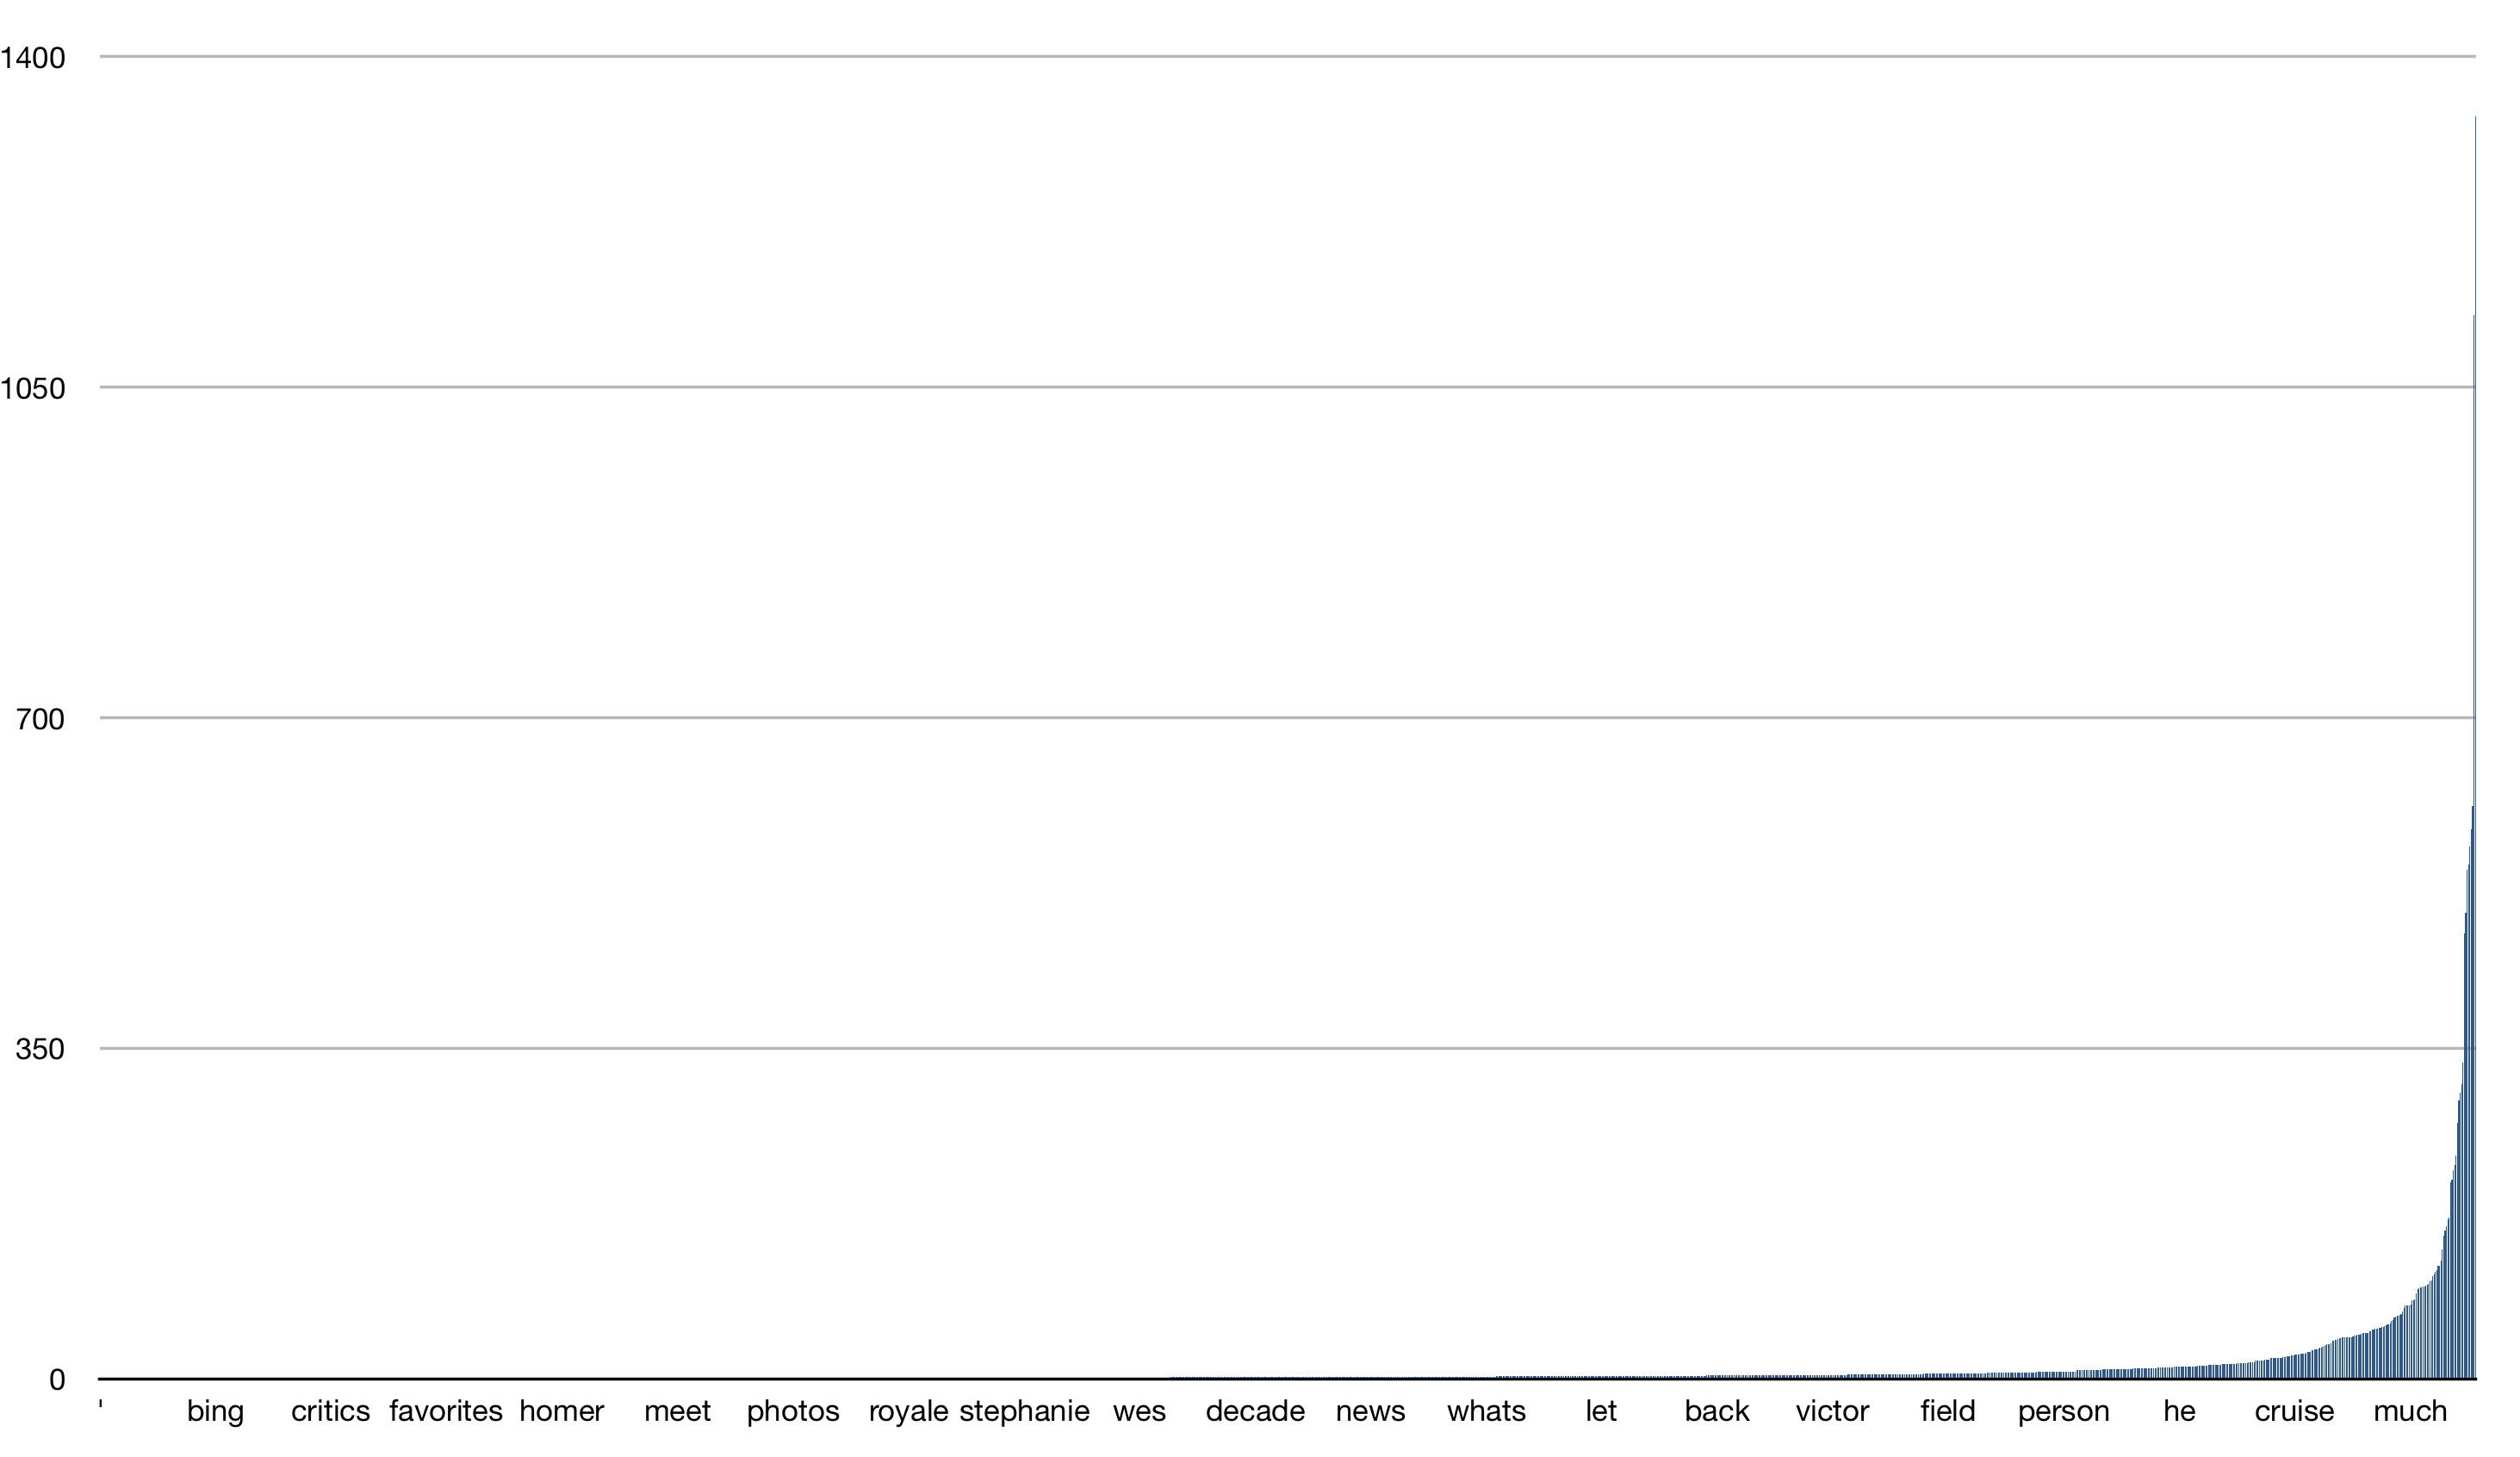
\includegraphics[width=\linewidth]{img/unigram.png}
  \caption{Zipf's law}
  \label{fig:unig}
\end{figure}

\subsection*{Language model}
To create a language model were employed two different tools: \textit{ngramcount} and \textit{ngrammake}. The first tool takes in input an archive of one or more FSTs and gives as output an FST representing the count of the n-grams. The resulting FST is used as input for \textit{ngrammake}. Both the tools allows to specify some parameters. To create different type of language models were specified the order of n-gram, for the first tool, and the smoothing method for the second tool. This allows to test multiple language models and search for the most precise one.
\subsection*{FST}
The FST was created using the lexicon and a file containing the matrix representation of the graph. Column one represent the start node, column two the end node, column three the token, column four the IOB-tag and column five the weight of the edge. The weight is computed as minus the logarithm of the probability of the \textit{bigram-token-tag}.
\subsection*{Testing}
Testing the language model and the FST  was  made creating a different file from the testset provided, containing in each row a whole sentence. Every line was transformed into an FST with multiple edges for the same couple of nodes, each of them weighted differently. After being composed with the trained FST and the language model, a shortest path algorithm is applied to the tested FST which results into a final FST with just one edge per couple of nodes. The file with the sentences was used for every type of FST and language model created before. 

\subsection*{Different training}
Since the number of tag \textit{O} is very large (figure \ref{fig:pos}), it's smart to associate the tag ``O`` with the related token. For instance, if the token is ``who``, the new tag will be ``O-who``. In this way the precision is improved. Although the algorithm for the creation of the language model and for the FST is the same, it was increased the range of the n-grams from 1-to-5 to 1-to-9.

\begin{figure}[ht]
  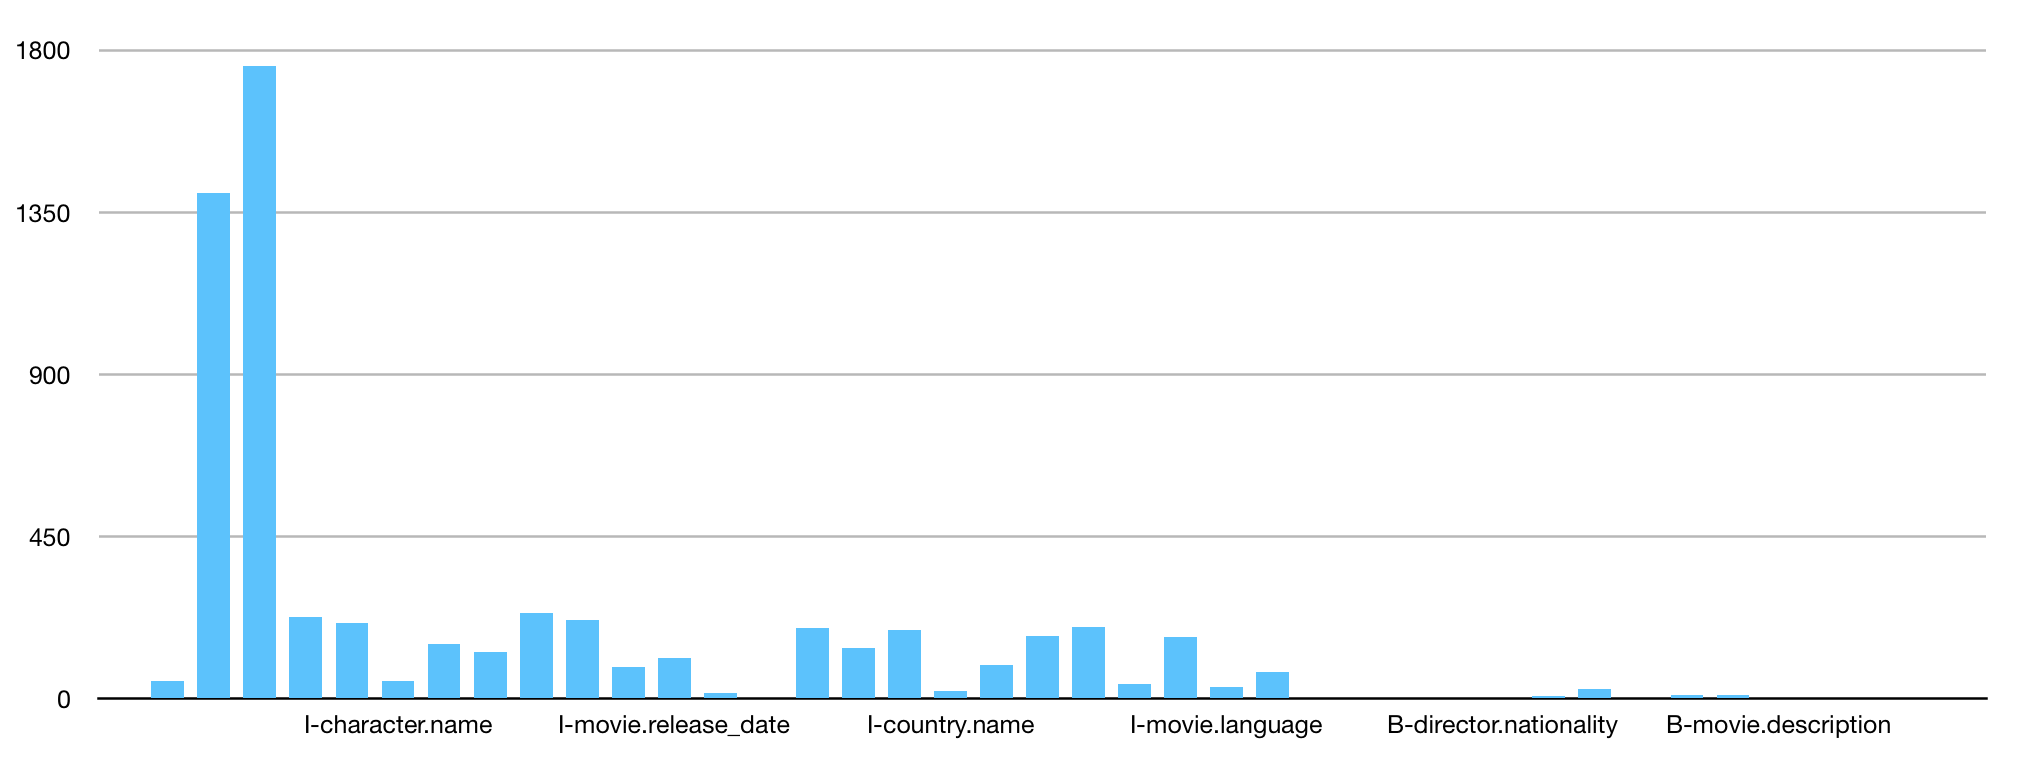
\includegraphics[width=\linewidth]{img/pos.png}
  \caption{POS-tags distribution}
  \label{fig:pos}
\end{figure}

\section{Evaluation}% (with Baseline)}
The evaluation is the last practical phase before the analysis of the reults. There are four tipes of results: true positive, true negative, false positive and false negative. Computing the accuracy is done dividing the summation of the correct decisions by the total amount of instances.
\begin{equation}
Accuracy= \frac{TP + TN} {TP + TN + FP + FN}
\end{equation}
Despite accuracy might seem to be enough, an unknown or infinite value of true negative can lead to a wrong result. Computing precision and recall is a good way to solve this problem.
\begin{equation}
Precision = \frac{TP} {TP + FP}
\end{equation}
\begin{equation}
Recall = \frac{TP}{TP + FN}
\end{equation}
 At this point it is possible to compute the harmonic mean of precision and recall, the F1 score.
 \begin{equation}
F1 =  \frac{2 * Precision * Recall}{Precision + Recall} 
\end{equation}
The output evaluation was made using a perl script called \textit{conlleval}, which takes in input a file containing for every line the token, the real POS-tag and the predicted one, each of them separated by a single space.
\subsection*{Evaluation on first type of language model}
Although conlleval gives all of the four types evaluation measures, the interesting result is the F1 score. On table \ref{f1-scores1} and \ref{f1-scores2} are listed the scores for each method and for each measure of n-gram. The results in bold are those that have passed the expeted performance. While comparing all method with each other the best one results to be ``witten bell``, comparing the different quantity of n-grams, \textit{n = 2} gives the best performance.
\begin{table}[ht]
\begin{center}
\begin{tabular}{|c|c|c|c|c|c|}
\hline
 & 1-gram & 2-gram & 3-gram \\ \hline
Absolute & 57.31 & \textbf{76.31} & 75.62  \\ \hline
Katz & 57.31 & 75.84 & 74.05 \\ \hline
Kneser-Ney & 57.31 & \textbf{76.27} & 75.67 \\ \hline
Unsmoothed & 57.31 & \textbf{76.15} & 75.46 \\ \hline
Presmoothed & 57.31 & \textbf{76.21} & 67.95 \\ \hline
Witten Bell & 57.31 & \textbf{76.31} & 75.52 \\ \hline
\end{tabular}
\caption{F1 Scores for every method and n-grams from 1 to 3}
\label{f1-scores1}
\end{center}
\end{table}


\begin{table}[ht]
\begin{center}
\begin{tabular}{|c|c|c|c|c|c|}
\hline
& 4-gram & 5-gram \\ \hline
Absolute & \textbf{76.04} & \textbf{76.00} \\ \hline
Katz & 73.12 & 63.19 \\ \hline
Kneser-Ney & \textbf{76.04} & \textbf{76.01} \\ \hline
Unsmoothed & 75.85 & 75.90 \\ \hline
Presmoothed & 67.01 & 66.75 \\ \hline
Witten Bell & \textbf{76.07} & \textbf{76.17} \\ \hline
\end{tabular}
\caption{F1 Scores for every method and n-gram 4 and 5}
\label{f1-scores2}
\end{center}
\end{table}

Figure \ref{fig:performance1} shows the learning scores for each method. For 1-gram and 2-gram the trend is almost the same for every method, but starting from 3-gram the performance go down, especially for ``katz`` and ``presmoothed``.
\begin{figure}[ht]
  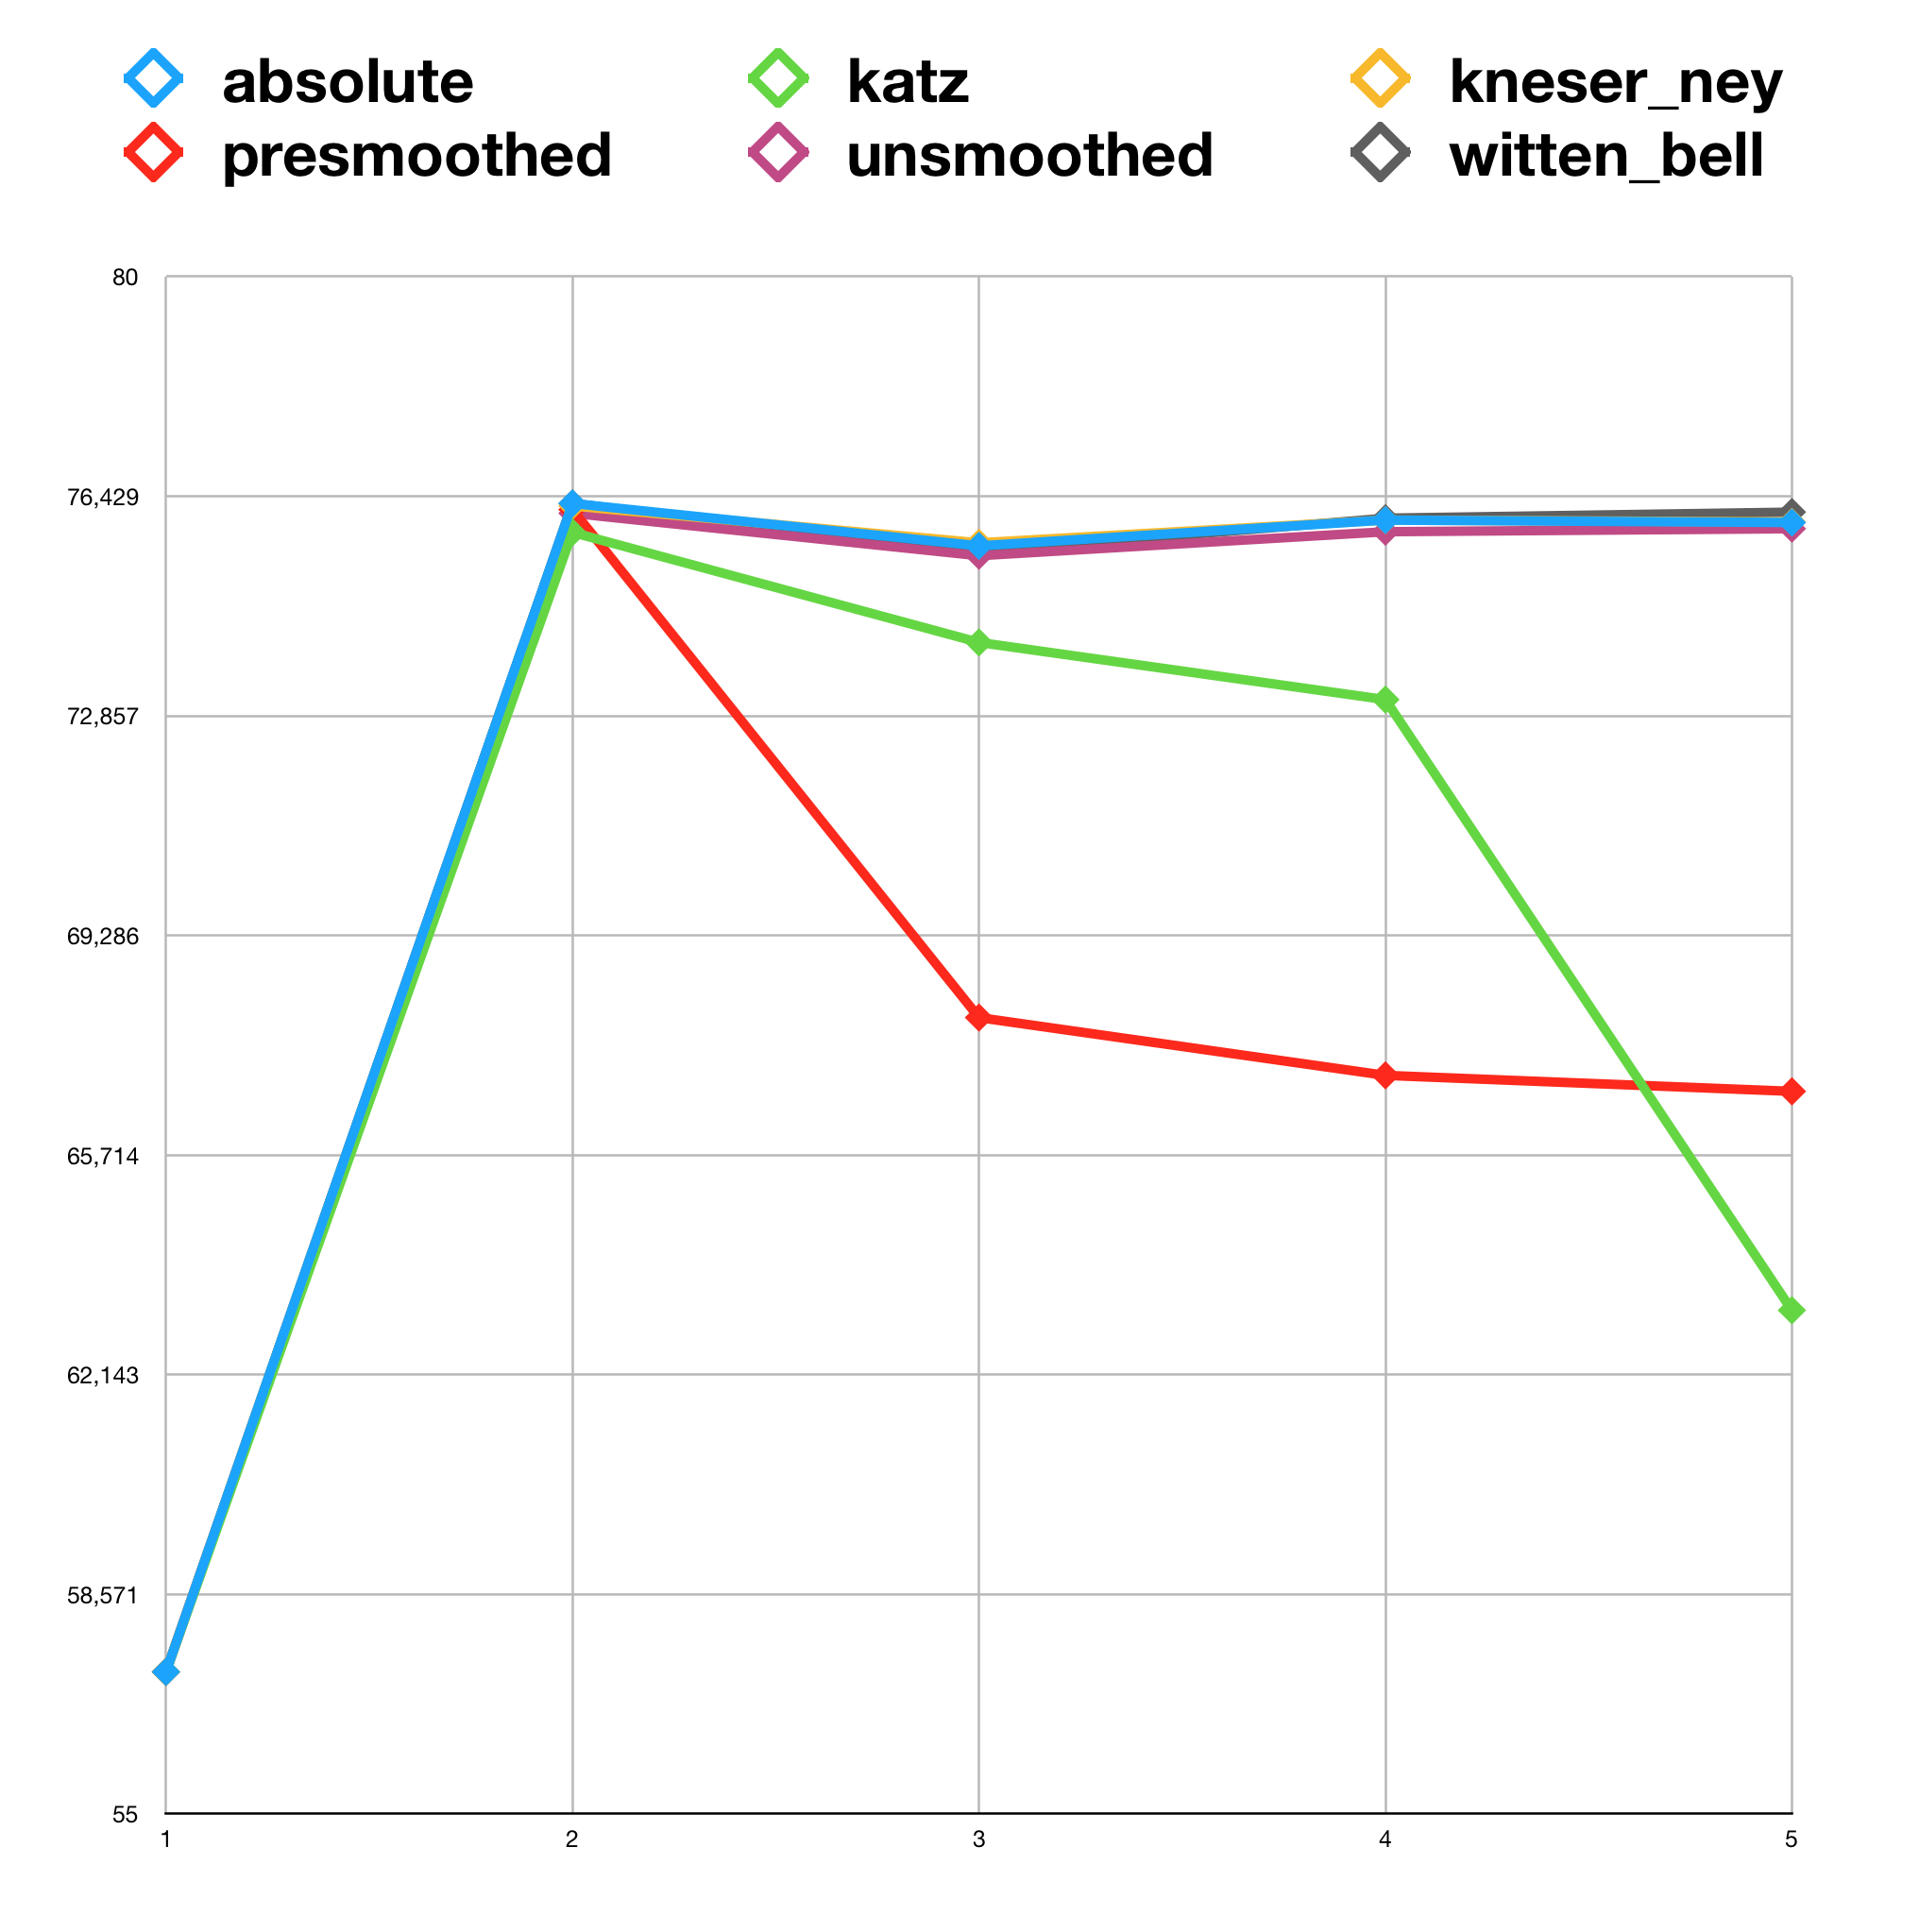
\includegraphics[width=\linewidth]{img/results.png}
  \caption{Performance trend for the first language model}
  \label{fig:performance1}
\end{figure}


\subsection*{Evaluation on second type of language model}
The language model trained over tags only shows higher performance with respect to the previous one. F1 scores for this language model are shown in table \ref{f1-o-scores-1}, \ref{f1-o-scores-2} and \ref{f1-o-scores-3}. The results in bold show that ``Kneser-Ney`` is the only method with F1 scores over the expected performance. Figure \ref{fig:performance2} shows that after 5-grams trend seems to be constant. 

\begin{table}[ht]
\centering
\begin{tabular}{|c|c|c|c|c|c|c|c|c|c|}
\hline
             & 1-gram & 2-gram & 3-gram  \\ \hline
absolute     & 55.31  & 78.88  & 81.37  \\ \hline
katz         & 55.31  & 78.64  & 80.85   \\ \hline
kneser\_ney  & 55.31  & 79.45  & \textbf{82.04} \\ \hline
presmoothed  & 55.31  & 77.61  & 79.54  \\ \hline
unsmoothed   & 55.31  & 76.14  & 78.45   \\ \hline
witten\_bell & 55.31  & 79.11  & 81.28  \\ \hline
\end{tabular}
\caption{F1 scores}
\label{f1-o-scores-1}
\end{table}

\begin{table}[ht]
\centering
\begin{tabular}{|c|c|c|c|c|c|c|c|c|c|}
\hline
              & 4-gram & 5-gram & 6-gram  \\ \hline
absolute     & 81.57  & 81.34  & 81.34   \\ \hline
katz           & 81.17  & 81.08  & 81.26    \\ \hline
kneser\_ney    & \textbf{82.69} &\textbf{82.37}  & \textbf{82.37}    \\ \hline
presmoothed  & 79.77  & 79.47  & 79.56   \\ \hline
unsmoothed     & 78.18  & 78.23  & 78.22   \\ \hline
witten\_bell & 81.37  & 81.21  & 81.07   \\ \hline
\end{tabular}
\caption{F1 scores for language model trained on tags only}
\label{f1-o-scores-2}
\end{table}
\begin{table}[ht]
\centering
\begin{tabular}{|c|c|c|c|c|c|c|c|c|c|}
\hline
              & 7-gram & 8-gram & 9-gram \\ \hline
absolute      & 81.43  & 81.52  & 81.52  \\ \hline
katz         & 81.17  & 81.08  & 81.08  \\ \hline
kneser\_ney  & \textbf{82.61}  & \textbf{82.61}  & \textbf{82.70}  \\ \hline
presmoothed  & 79.56  & 79.56  & 79.56  \\ \hline
unsmoothed   & 78.45  & 78.77  & 78.58  \\ \hline
witten\_bell & 81.52  & 81.48  & 81.48  \\ \hline
\end{tabular}
\caption{F1 scores for language model trained on tags only}
\label{f1-o-scores-3}
\end{table}
\begin{figure}[ht]
  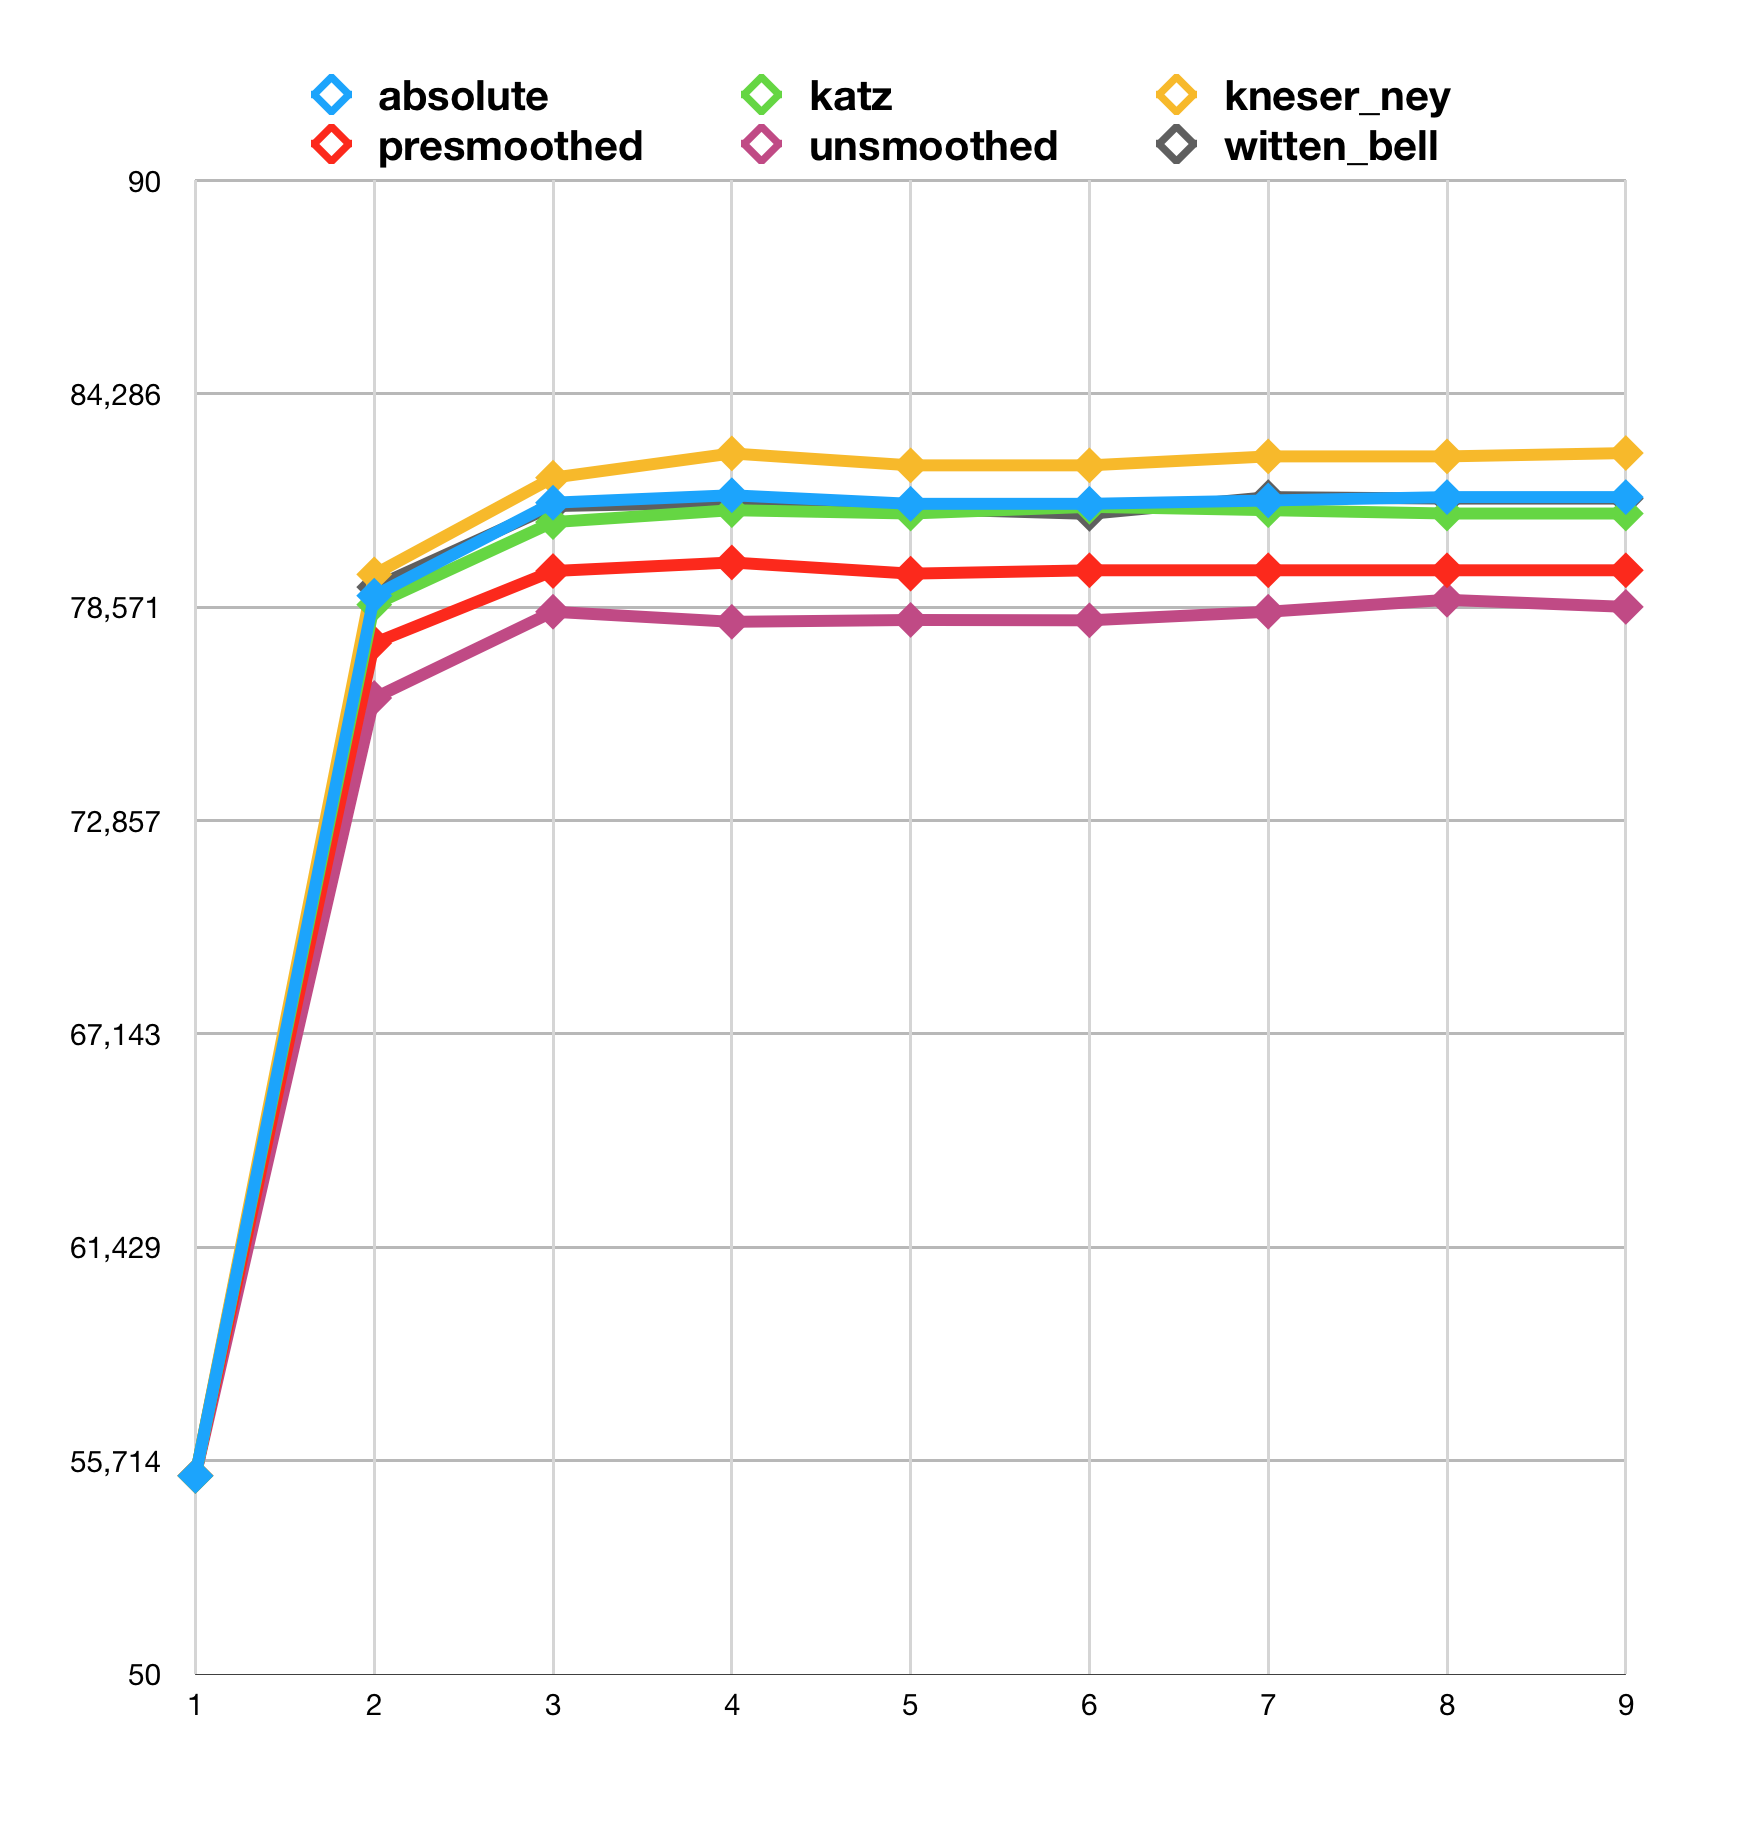
\includegraphics[width=\linewidth]{img/results-o.png}
  \caption{Performance trend for the second language model}
  \label{fig:performance2}
\end{figure}

\section{Conclusion}
The language models trained for this project are two. The first one was trained over the dataset as it was provided, while the second one was trained over a modified dataset, which containes only tags. The second language model has better performance with respect to the first one and the F1 score remains almost constant from 5-gram up to 9-gram. This means that quality is not improved just by increasing n-grams.


\end{document}
